\documentclass{article}
\usepackage[UTF8]{ctex}
\usepackage{CJKutf8}
\usepackage{color}
\usepackage{natbib}
\usepackage{graphicx}
\usepackage{subfigure}
\usepackage{geometry}
\usepackage{amsmath}
\usepackage{mathrsfs}
\usepackage{algorithm}  
\usepackage{algorithmicx}  
\usepackage{algpseudocode}
\usepackage[backref]{hyperref}
\usepackage{diagbox}
\usepackage{pythonhighlight}
\hypersetup{hidelinks}
\renewcommand{\algorithmicrequire}{\textbf{Input:}}  % Use Input in the format of Algorithm  
\renewcommand{\algorithmicensure}{\textbf{Output:}}
\geometry{a4paper, scale=0.8}

\title{\textbf{EE447 Homework2 \\ Double-Spend Problem}}
\author{付昊源 517021910753}
\date{April 24, 2020}

\begin{document}

\maketitle

%%%%%%%%%%%%%%%%%%%%%%%%%%%%%%
\section*{Problem Statement}
Suppose that the longest chain of a blockchain is confirmed every time a block is received. According to the longest chain principle of the blockchain, the confirmed blocks on the chain may be abandoned due to the extension of other branches. This is a common double-spend problem in blockchain. In order to deal with this problem, people put forward the concept of "k confirmation transaction", which means that after a transaction is listed on the chain, it will get k confirmations on the blockchain before it is formally closed.

It is known that the cost per unit time for an attacker to obtain 51\% of the computing power in the blockchain is 10,000 yuan, and the probability of successfully generating a block on the target branch in a unit time is 51\% (if the unit time attacks The block generation fails, others will generate a block on the main chain successfully). There is an existing transaction worth 1 million yuan waiting to be completed. At least how many confirmations must be obtained after the transaction is chained to ensure that the expected value of the cost of using 51\% of the computing power to tamper the transaction is higher than the transaction amount?

\section*{Solution}
\subsection*{Formulation}
According to the "k confirmation transaction", there will be k confirmations, which means there will be at least $k(k\ge 0)$ extra blocks linked to the master chain before the attacker starts making fake blocks. Thus, after the confirmation, the current block chain is shown as Figure 1.
\begin{figure}[h]
    \centering
    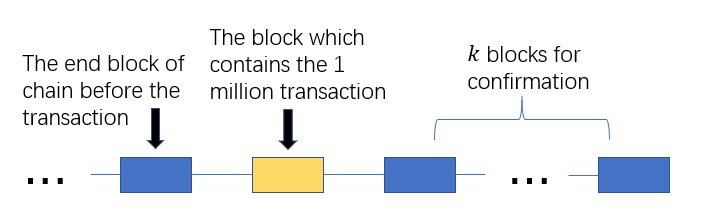
\includegraphics[width=0.6\linewidth]{HW2_1.PNG}
    \caption{The current block master chain after $k$ confirmations.}
\end{figure}

It is also at this time that the attacker starts building fake blocks to eliminate the 1 million transaction. However, the attacker cannot always successfully generate a new block, and there will be new blocks linked to the original chain. Let's assume $x(x\ge 0)$ extra blocks are linked to the original chain after the attacker starts attacking. Suppose the attacker successfully creates a new branch at last, and the final state of block chain will be shown as figure 2.
\begin{figure}[h]
    \centering
    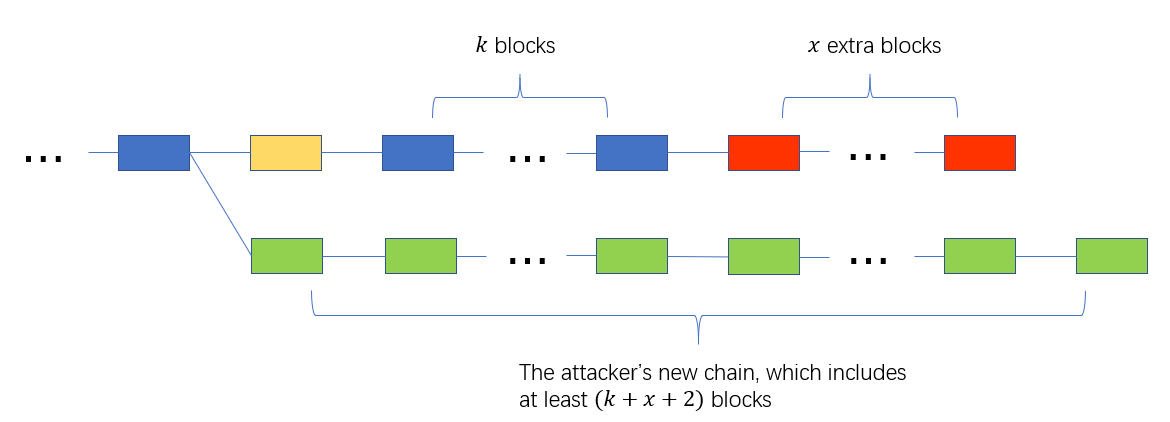
\includegraphics[width=0.9\linewidth]{HW2_2.PNG}
    \caption{The final state of blockchain, assuming the attacker successfully add a new branch.}
\end{figure}

\subsection*{Calculating Process}
According to the formulation above, we can get the result that there will be $(k+2x+2)$ time units for the attacker to hold 51\% computing power, which means the total cost will be $(k+2x+2)$ money units (a money unit is 10,000 yuan) in case of $x$ extra blocks. So the next step is to calculate the probability $p(x)$ of $x$ extra blocks linked to the initial chain. And we can get the expected value of cost by
\begin{equation}
    E(cost)=\sum_{x=1}^{\infty} p(x)\cdot (k+2x+2)
\end{equation}

Then let's talk about how to calculate term $p(x)$. We know that in the period of $(k+2x+2)$ time units, the attacker succeeds for $(k+x+2)$ times while he fails for $x$ times. So if we can get the permutation value $c(k,x)$, which means there are $c(k,x)$ types of permutations satisfying the parameter $k$ and $x$, we can calculate $p(x)$ by
\begin{equation}
    p(x)=c(k,x)\cdot 0.51^{k+x+2}\cdot 0.49^{x}
\end{equation}
since the attacker succeeds with probability 51\% and fails with probability 49\%.

For term $c(k,x)$, it counts any possible permutation with $(k+x+2)$ success and $x$ failure, under the constrain that at any time except the final state, the length of new branch cannot exceed the original one. This is because, if any time the new branch is longer, it can be the main chain and the attacker has already succeeded. Actually, $c(k,x)$ is hard to get by formulation, but easy to get using recursive function in python. I will show my python codes in next page.
\newpage
\begin{python}
from scipy.special import comb

dp = {}

def combinations(ahead, X):
    '''
    ahead means how many blocks of the initial chain is ahead of the attacker's new chain
    x means how many blocks will be linked to the initial chain
    '''
    if X == 0:
        return 1

    has_key = False
    if ahead in dp.keys():
        has_key = True
        if X in dp[ahead].keys():
            return dp[ahead][X]
    
    res = 0
    for x in range(1, X + 1):
        if x > ahead + 1:
            break
        res += comb(ahead + 1, x) * combinations(2 * x - 1, X - x)
    
    if has_key:
        dp[ahead][X] = res
    else:
        dp[ahead] = {X: res}
    return res
\end{python}

The basic idea is, each time we get the length of original chain ahead of new chain and how many blocks will be linked to the original chain, we know that in the following $ahead+1$ times, there will be at least $1$, at most $\min\{x,ahead+1\}$ blocks linked to original chain. Then we recompute the value of $ahead$ and $x$, recursively calculating.

\subsection*{Conclusion: $k=10$}
With the help of equations above and Python code, I can test different $k$ and $x$ to calculate expected value of total cost. In real test, I set $x\in[0,200]$ and try different $k$. I find $k=10$ is the first time that $E(cost)$ has first come above 100, which is the transaction amount. So I think $k=10$ is my answer and people should feel safe if they wait for 10 blocks to confirm.

However, in theory we should accumulate all integer $x\in[0,+\infty)$, but we can only add finite numbers of $x$ under the constrain of programming. Though this may not give the very exact answer, but I think this answer is resonable. In real situation, an attacker won't spend too much time units to attack. In this problem, the attack won't spend more than 100 time units to attack, because even if he succeeds finally, he will lose more than 100 units of money.

There is another method: simulating this process. This method is easy to understand, but it strongly depends on probability and cannot get the exact expected value. I still think computing in theroy is more trust-worthy.

In the following, I will show the main function codes for testing my solution and I also show some results about different $k$ and $x$ in Table 1.

\begin{python}
def main():
    k = 7 # changable
    X = 150 # changable
    p = 0.51
    E = 0.0
    for x in range(X + 1):
        tmp = (k + 2 * x + 2) * combinations(k + 1, x)
        tmp *= (p ** (k + x + 2))
        tmp *= ((1 - p) ** x)
        E += tmp
    print(E)
\end{python}

\begin{table}[h]
    \centering
    \begin{tabular}{cccccc}
        \hline
        \diagbox{$x$}{$E(cost)$}{$k$} & 7 & 8 & 9 & 10 & 11 \\
        \hline
        150 & 71.5483 & 74.2677 & 76.1859 & 77.3711 & 77.8910 \\
        200 & 90.4091 & 95.0620 & 98.8229 & {\color{red}101.7471} & 103.8900 \\
        250 & 107.1623 & 113.6434 & 119.1838 & 123.8276 & 127.6205 \\
        300 & 122.2776 & 130.4729 & 137.7025 & 144.0023 & 149.4093 \\
        \hline
    \end{tabular}
    \caption{The expected value of total cost with different $k$ and $x$.}
\end{table}


%%%%%%%%%%%%%%%%%%%%%%%%%%%%%%

\end{document}
